\documentclass{ltjbook}
\usepackage{docmute} 
\usepackage{../../myStyle} 

\begin{document}

\chapter{F検定/分散分析の基礎}
\label{ch19_Ftest}

ここまでは要因計画に基づき，全体の平方和を効果と誤差に分解する方法についてみてきました。今回はこれに帰無仮説検定の考え方を加えます。つまり，効果の大きさが誤差に比べてどれほど大きいかを評価し，その大きさが偶然にしては珍しいものであるかどうかを「判断する」ことについて考えていきたいと思います。

この検定方法は\keyterm{F検定}{Fけんてい}{F test}と呼ばれます。検定統計量として$F$分布と呼ばれる分布を使うからです。別名で\keyterm{分散分析}{ぶんさんぶんせき}{ANalysis Of VAriance;ANOVA}とも呼ばれます。注意して欲しいのは，分散を使った分析なので分散分析という名前がついていますが，目的はあくまでも群間の\textbf{平均値}に差があるかどうかを判断するために使うものであるということです。


ここにあるように，まずは前期でやった線形モデルのことをよく思い出していただく必要があります。その上で，効果や誤差の「大きさ」として計算された平方和の比が従う分布を利用して，検定と接合することになります。検定は帰無仮説と対立仮説の勝負による判定にすぎないことに注意しつつ，また何が帰無仮説として置かれていたのかに注意して読み進めてください。

\section{検定統計量の算出}
ここまで行ってきた平方和の分解について，改めて確認しておきましょう。

まず要因による操作がなければ，すべてのデータは全体平均に一致すると考えたのでした。そこで全体平均から群平均の差分が効果，各データ点から群平均の差分が誤差と考えました。各データ点から全体平均の差分の二乗和が全体の平方和(=$SS_T$)であり，これを効果の平方和(=$SS_A$)と誤差の平方和(=$SS_E$)に分解したのでした。

$$SS_T = SS_A + SS_E$$

要因の数が増えても基本的には同じですが，要因が2つ以上ある場合は「水準の組み合わせによる特別な効果」，すなわち交互作用も考慮する必要があるのでした。これを踏まえて，2要因の場合は次のように表されるのでした。

$$SS_T = SS_A + SS_B + SS_{AB} + SS_E$$

ここでは交互作用を$SS_{AB}$と表しています。平方和の分解は要因の数に応じて複雑になりますが，基本的な考え方は同じです。

さて，この誤差に対して効果が十分大きいか，ということを考えます。効果が大きいとは，群平均が全体平均から大きく離れていることを意味します。つまり，$SS_A$が大きいことを意味します。しかし，$SS_A$が大きいか小さいかは，そのままではわかりません。なぜなら，$SS_A$はデータの数に依存するからです。データ数が多ければ，それだけ$SS_A$も大きくなります。同様に，$SS_E$もデータ数に依存します。ここで知りたいのは，平方和の絶対的な大きさの大小ではなく，「群間のばらつきが，群内のばらつきに比べてどれほど大きいか」という相対的な大きさであり，$SS_A$や$SS_E$の大きさを生んだ群の水準1つあたりの影響力を考える必要があります。

分散は平方和を足した数で割ったものでした\footnote{思い出しましょう。$$\hat{\sigma^2} = \frac{1}{n-1}\sum (x_i - \bar{x})^2$$ですね。}。ここでの$SS_A,SS_E$はまだ平方和(Sum of Squares)の段階で，足した数で割ったものになっていません。また，推測統計学ですから標本分散ではなく不偏分散で考えますので，$n-1$，すなわち自由度で割ることになります。

平方和(Sum of Squares)を自由度(degrees of freedom)で割ったものを\keyterm{平均平方}{へいきんへいほう}{Mean Squares}と呼びます。この平均平方を使って，効果の大きさが誤差に比べてどれほど大きいかを評価します。これがF検定です。

F検定で用いられる検定統計量$F$は，\keyterm{F分布}{Fぶんぷ}{F distribution}に従います。F分布は簡単にいうと，分散の比の分布です。誤差に比べて効果がどれだけ大きいかが知りたいのですから，丁寧にいうならば「誤差1水準の平均平方に対する効果1水準の平均平方の比」を考えることになります。F分布は，分子(効果)と分母(誤差)の2つの自由度を持つ分布であることに注意してください。

では具体的な数字とともに，また帰無仮説検定の流儀に習って，順に計算ステップを見ていきましょう。

\section{分散分析の手順}
数値例として，第\ref{ch17_RCT}講，セクション\ref{Design_effect}(Pp.\pageref{Design_effect})で用いたデータを使います。全体平均は5.25であり，表\ref{tbl:19_01}にあるように，効果と誤差に分解した結果，$SS_T=18.25,SS_A=6.50,SS_E=11.75$となりました。合計欄の(T)の二乗，(A)の二乗，(E)の二乗の合計がそれぞれ$SS_T,SS_A,SS_E$で，$SS_T=SS_A+SS_E$となっていることを確認してください。

\begin{table}[ht]
	\centering
	\caption{一要因3水準，Betweenデザインのデータ例(再掲)}
	\begin{tabular}{cccrrrrrrr}
		\hline
		ID & 水準 & value & 平均偏差(T)   & 群の効果(A)   & 誤差(E)     & (T)の二乗 & (A)の二乗 & (E)の二乗 \\
		\hline
		1 & 毎日 & 6 & 0.75  & 0.25  & 0.50  & 0.562   & 0.062 & 0.250 \\
		2 & 毎日 & 6 & 0.75  & 0.25  & 0.50  & 0.562   & 0.062 & 0.250 \\
		3 & 毎日 & 5 & -0.25 & 0.25  & -0.50 & 0.062   & 0.062 & 0.250 \\
		4 & 毎日 & 5 & -0.25 & 0.25  & -0.50 & 0.062   & 0.062 & 0.250 \\
		5 & ときどき & 7 & 1.75  & 0.75  & 1.00  & 3.062   & 0.562 & 1.000 \\
		6 & ときどき & 4 & -1.25 & 0.75  & -2.00 & 1.562   & 0.562 & 4.000 \\
		7 & ときどき & 7 & 1.75  & 0.75  & 1.00  & 3.062   & 0.562 & 1.000 \\
		8 & ときどき & 6 & 0.75  & 0.75  & 0.00  & 0.562   & 0.562 & 0.000 \\
		9 & あげない & 4 & -1.25 & -1.00 & -0.25 & 1.562   & 1.000 & 0.062 \\
		10 & あげない & 3 & -2.25 & -1.00 & -1.25 & 5.062   & 1.000 & 1.562 \\
		11 & あげない & 4 & -1.25 & -1.00 & -0.25 & 1.562   & 1.000 & 0.062 \\
		12 & あげない & 6 & 0.75  & -1.00 & 1.75  & 0.562   & 1.000 & 3.062 \\
		\hline\hline
		 & & 合計 & 0.00   & 0.00   & 0.00   & 18.25   & 6.50  & 11.75 \\\hline
	\end{tabular}
	\label{tbl:19_01}
\end{table}

さて，このデータから(水やりの)効果が誤差に比べて十分大きいかどうかを「判断」しましょう。

帰無仮説検定の手順をもう一度確認しておきます。不安な人は第\ref{ch13_NHST}講，セクション\ref{sec:13_02}(Pp.\pageref{sec:13_02})を読み返してください。
\begin{enumerate}
	\item 仮説を設定する。
	\item 統計的仮説検定に用いられる検定統計量を選択する。
	\item 仮説選定判断の基準になる確率を設定する。
	\item 実際のデータから検定統計量の実現値を計算する。
	\item 最初に定めた仮説を支持するかどうかを判断する。
\end{enumerate}

\paragraph{仮説の設定}帰無仮説と対立仮説が必要です。対立仮説は「効果があった」ということですから，帰無仮説は「効果がなかった」という仮説であり，この2つの仮説を戦わせることになります。

今回，効果がなかったというのはどのように考えれば良いでしょうか。効果がなかったというのは，群平均に差がなかった，すなわちすべてが全体平均に等しかったということです。仮説は母数に対して立てるものですから，帰無仮説は母平均に差がない，ということになります。数学的に書くなら，三つの群の平均が次のようになっていることを意味します。
$$H_0 : \mu_1 = \mu_2 = \mu_3$$
そして対立仮説はこれの否定，ということになります。

ところで，勘の良い人はここで「おや，まてよ？ 」と思うかもしれません。そうです，この帰無仮説，いろんな否定の仕方が考えられるのです。つまり，
\begin{itemize}
	\item $\mu_1 \neq \mu_2$だけど，$\mu_3$については$\mu_1=\mu_3$なのか$\mu_2=\mu_3$なのかわからない。
	\item $\mu_1 \neq \mu_3$だけど，$\mu_2$については$\mu_1=\mu_2$なのか$\mu_3=\mu_2$なのかわからない。
	\item $\mu_2 \neq \mu_3$だけど，$\mu_1$については$\mu_2=\mu_1$なのか$\mu_3=\mu_1$なのかわからない。
	\item $\mu_1 \neq \mu_2 \neq \mu_3$，つまりとにかく全部違う
\end{itemize}
の4パターン考えられます。実はこれ，すべて対立仮説の一員なのです。帰無仮説は一人でこれらに立ち向かうことになります。
\paragraph{検定統計量を選択}平均値の推定ですが，分散を検定対象にするので$F$分布というものを使うのでした。検定統計量は$F$値になります。
\paragraph{判断の基準になる確率を設定}有意水準$\alpha$，今回も5\%で勝負を決めるとしましょう。
\paragraph{検定統計量の実現値を計算}
では実際に$F$値を計算してみましょう。
効果の平方和$SS_A$は6.50，誤差の平方和$SS_E$は11.75でした。これを自由度で割って平均平方を求めます。

群の効果は，3つの水準でこの平方和を作り出したわけですから，一単位は$3-1=2$で考えて，MSは
\[ 6.50 / (3-1) = 3.250\]
となります。また，誤差の一単位あたりの大きさは，各群の平均と各値の差分で作られており，各群に4人配置されていますから，各群の誤差の自由度($4-1$)が3群あると考えて
\[ 11.75/3(4-1)=11.75/9 = 1.306\]
です。

F分布に従う検定統計量は，このMSの比率です。ここでは「誤差に比べてどれぐらい効果が大きかったか」がみたいのですから，効果のMSを誤差のMSで割って$F$値を算出します。
具体的には，
\[F = 3.250/1.306 = 2.489\]
ということになります。

$F$値はF分布に従います。比の分布なので，分布の形状を決める自由度は分子と分母の2つが必要です。自由度は先ほどの一単位を計算した値であり，分子の自由度$df_1 =2$，分母の自由度$df_2 = 9$の$F$分布からその出現確率を計算し，これが0.1379077と出ます\footnote{RでF分布の確率関数は\texttt{f}ですから，\texttt{1-pf(2.489,df1=2,df2=9)}として算出します。}。これは5\%よりも大きい値でしたので，統計的に有意とは判断できない(帰無仮説を棄却できない)ことになります。

\paragraph{分散分析表}
計算ステップは複雑に見えますが，実際は計算機が計算してくれます。また，結果がわかりやすくなるように，次のような\keyterm{分散分析表}{ぶんさんぶんせきひょう}{ANOVA Table}にまとめて報告することが一般的です(表\ref{tbl:19_02})。
\begin{table}[ht]
	\centering
	\caption{ANOVA Table}
	\begin{tabular}{lrrrrr}
		\hline
		          & Df & SS     & MS    & F value & $p$   \\
		\hline
		condition & 2  & 6.500  & 3.250 & 2.489   & 0.138 \\
		Residuals & 9  & 11.750 & 1.306 &         &       \\
		\hline
	\end{tabular}
	\label{tbl:19_02}
\end{table}

この表にあるように，平方和(SS)$\to$自由度(df)をつかって平均平方(MS)$\to$比率のF比$\to$$p$値の計算，という流れになっていることを確認してください。

結果をレポートなどで報告するときは，この表とともに，
\begin{quote}
	一要因3水準の分散分析を行ったところ，$F(2,9)=2.489,p=0.138$で，水準間に統計的に有意な差はみられなかった。
\end{quote}
などと表記します。


\subsection{効果量は?}
帰無仮説検定で，差があったかなかったか，という判断だけで終わらせるのではなく，どの程度の差があったのかについて報告しないといけないのでした。分散分析における効果量は，全体の分散のうち効果の分散がどれほどの量であったかという比率，つまり効果量=効果の分散/全体の分散=1 - (誤差の分散/全体の分散),で算出できます。これを$\varepsilon^2$(イプシロンの二乗)といいます\footnote{他にも同じような意味を持つ$\eta^2$という指標もよく使われます。}。

とはいえ，母集団における効果の分散，母集団における誤差の分散は分かりませんので，標本の不偏分散をつかって標本効果量として推定するしかありません。今回，全体の標本(不偏)分散は，表\ref{tbl:19_01}の「(T)の二乗」列の一番下にある18.25，これを$12-1=11$で割った$18.25/11=1.659091$ですから，

\[\varepsilon^2 = 1 - \frac{1.306}{1.659} = 0.2127788 \]

となりました。合わせて報告した方が良いでしょう。


\section{線形モデルとしてみた分散分析}

ここで，帰無仮説検定の側から線形モデルを見てみましょう。
平方和の分解が線形モデルと同じだ，ということはすでに指摘した通りです(セクション\ref{experiment_is_lm},Pp.\pageref{experiment_is_lm})。個々の値 = 全体平均 + 効果 + 誤差という式を記号で書けば，$y_i = b_0 + b_1x_{1i} + e_i$という線形モデルの式と同じ，$b_0$は全体平均，$b_1x_{1i}$が効果，$e_i$が誤差に対応しますよね。一要因の分散分析は単回帰モデルですし，二要因の分散分析は重回帰モデルです。

さて，帰無仮説検定の話をしたときに，これはモデル比較だと言いました($\to$セクション\ref{sec:13_02}，Pp.\pageref{sec:13_02})。帰無仮説というモデル，対立仮説というモデルを比較して，どちらに軍配を上げるかという勝負判定をする，これが帰無仮説検定だと。

ここでの「モデル」という言葉は，たとえば帰無仮説は$\mu_1 - \mu_2 =0$とおく，といった表現がなされますから，前期の(線形)モデルという表現と異なるイメージを持ったかもしれません。しかしこれもモデル，しかも線形のモデルなのです。今からこの「帰無仮説検定」と「線形モデル」を概念的に統合することを説明してきます。

そのための例として，次のようなデータを用意しました(図\ref{fig:19_01})。これは対応のない，2つの群(仮に実験群と統制群とします)の平均値をプロットしたものです。ここで示されている平均値は標本平均ですから，そこに差があるのは見た通りです。ちなみに黒い点は各群における個体1つ1つの観測値です。

\begin{figure}[ht]
	\centering
	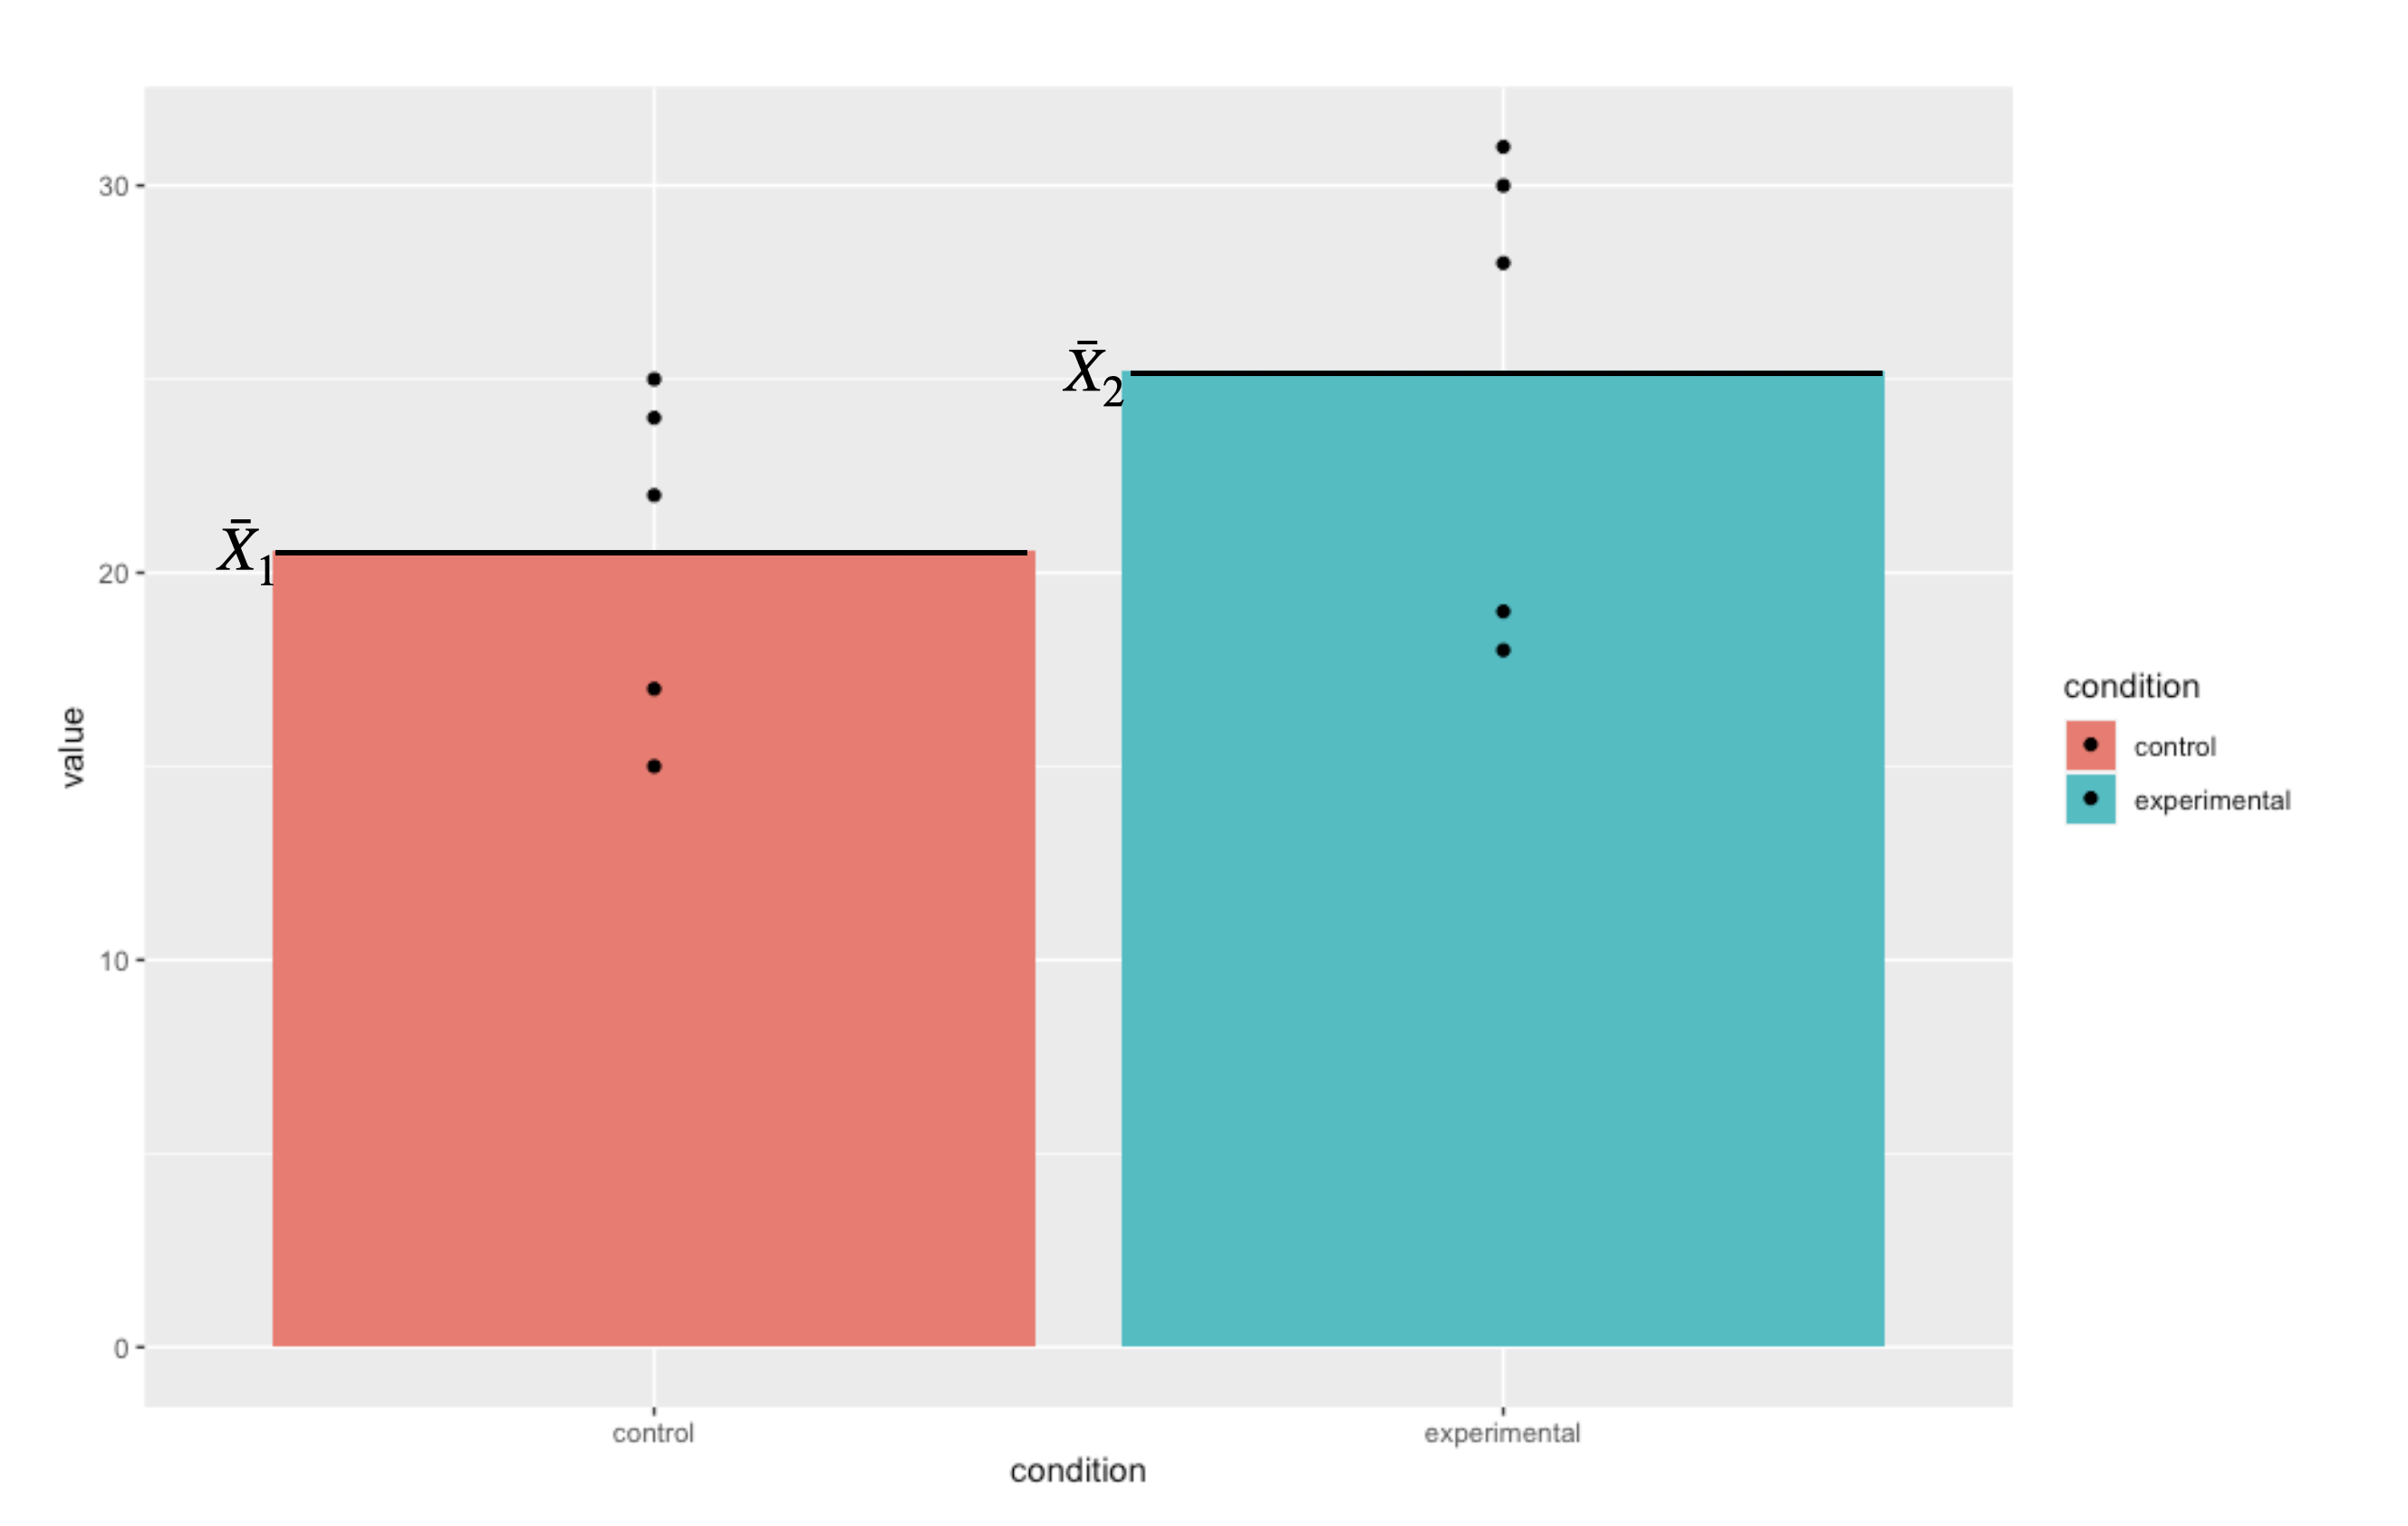
\includegraphics[keepaspectratio,width=0.75\linewidth]{figures/19_Ftest/two_levels.png}
	\caption{2つの群の平均値のプロット。黒い点は各群のそれぞれの観測値}
	\label{fig:19_01}
\end{figure}

このデータを別の見方で捉えてみましょう。

今回の例において，従属変数である心理変数はどういう特徴なのか，目に見えないものなのでわかりません。でも，心の問題は無数の要因が積み重なった結果であると考えると，正規分布を仮定するのが自然です。つまり，実験群のひとも統制群のひとも，大きな視点から考えれば同じ人間という正規母集団からのサンプルなのです。

さて，実験参加者たちは実験者によって無作為に実験群と統制群に割り当てられました(RCT)。個人差がなければ，各群1名ずつのスコアを比較して考えれば良いのですが，人間を対象にしている以上そうはいきません。個人差がどうしても生じてしまうので，複数人を集めて個人差を相殺することを考えます。各群の平均値の違いを見ることで，操作の効果を見ることにするのです。

もしこの実験に効果がなければ，2群の平均値は同じになるでしょう。この時の平均値は，実験群と統制群に分けた効果がないのですから，両群のスコアを足しあわせた全体平均になるはずです。効果がない=全体平均，なのです。しかし，群ごとに見てみると全体平均から違いが生じています。図\ref{fig:19_02}では，統制群は相対的に低く，実験群は相対的に高い平均値を示しています。この差分こそ(図\ref{fig:19_02}では短い緑の矢印で示しています)，実験の効果なのです。

\begin{figure}[hb]
	\centering
	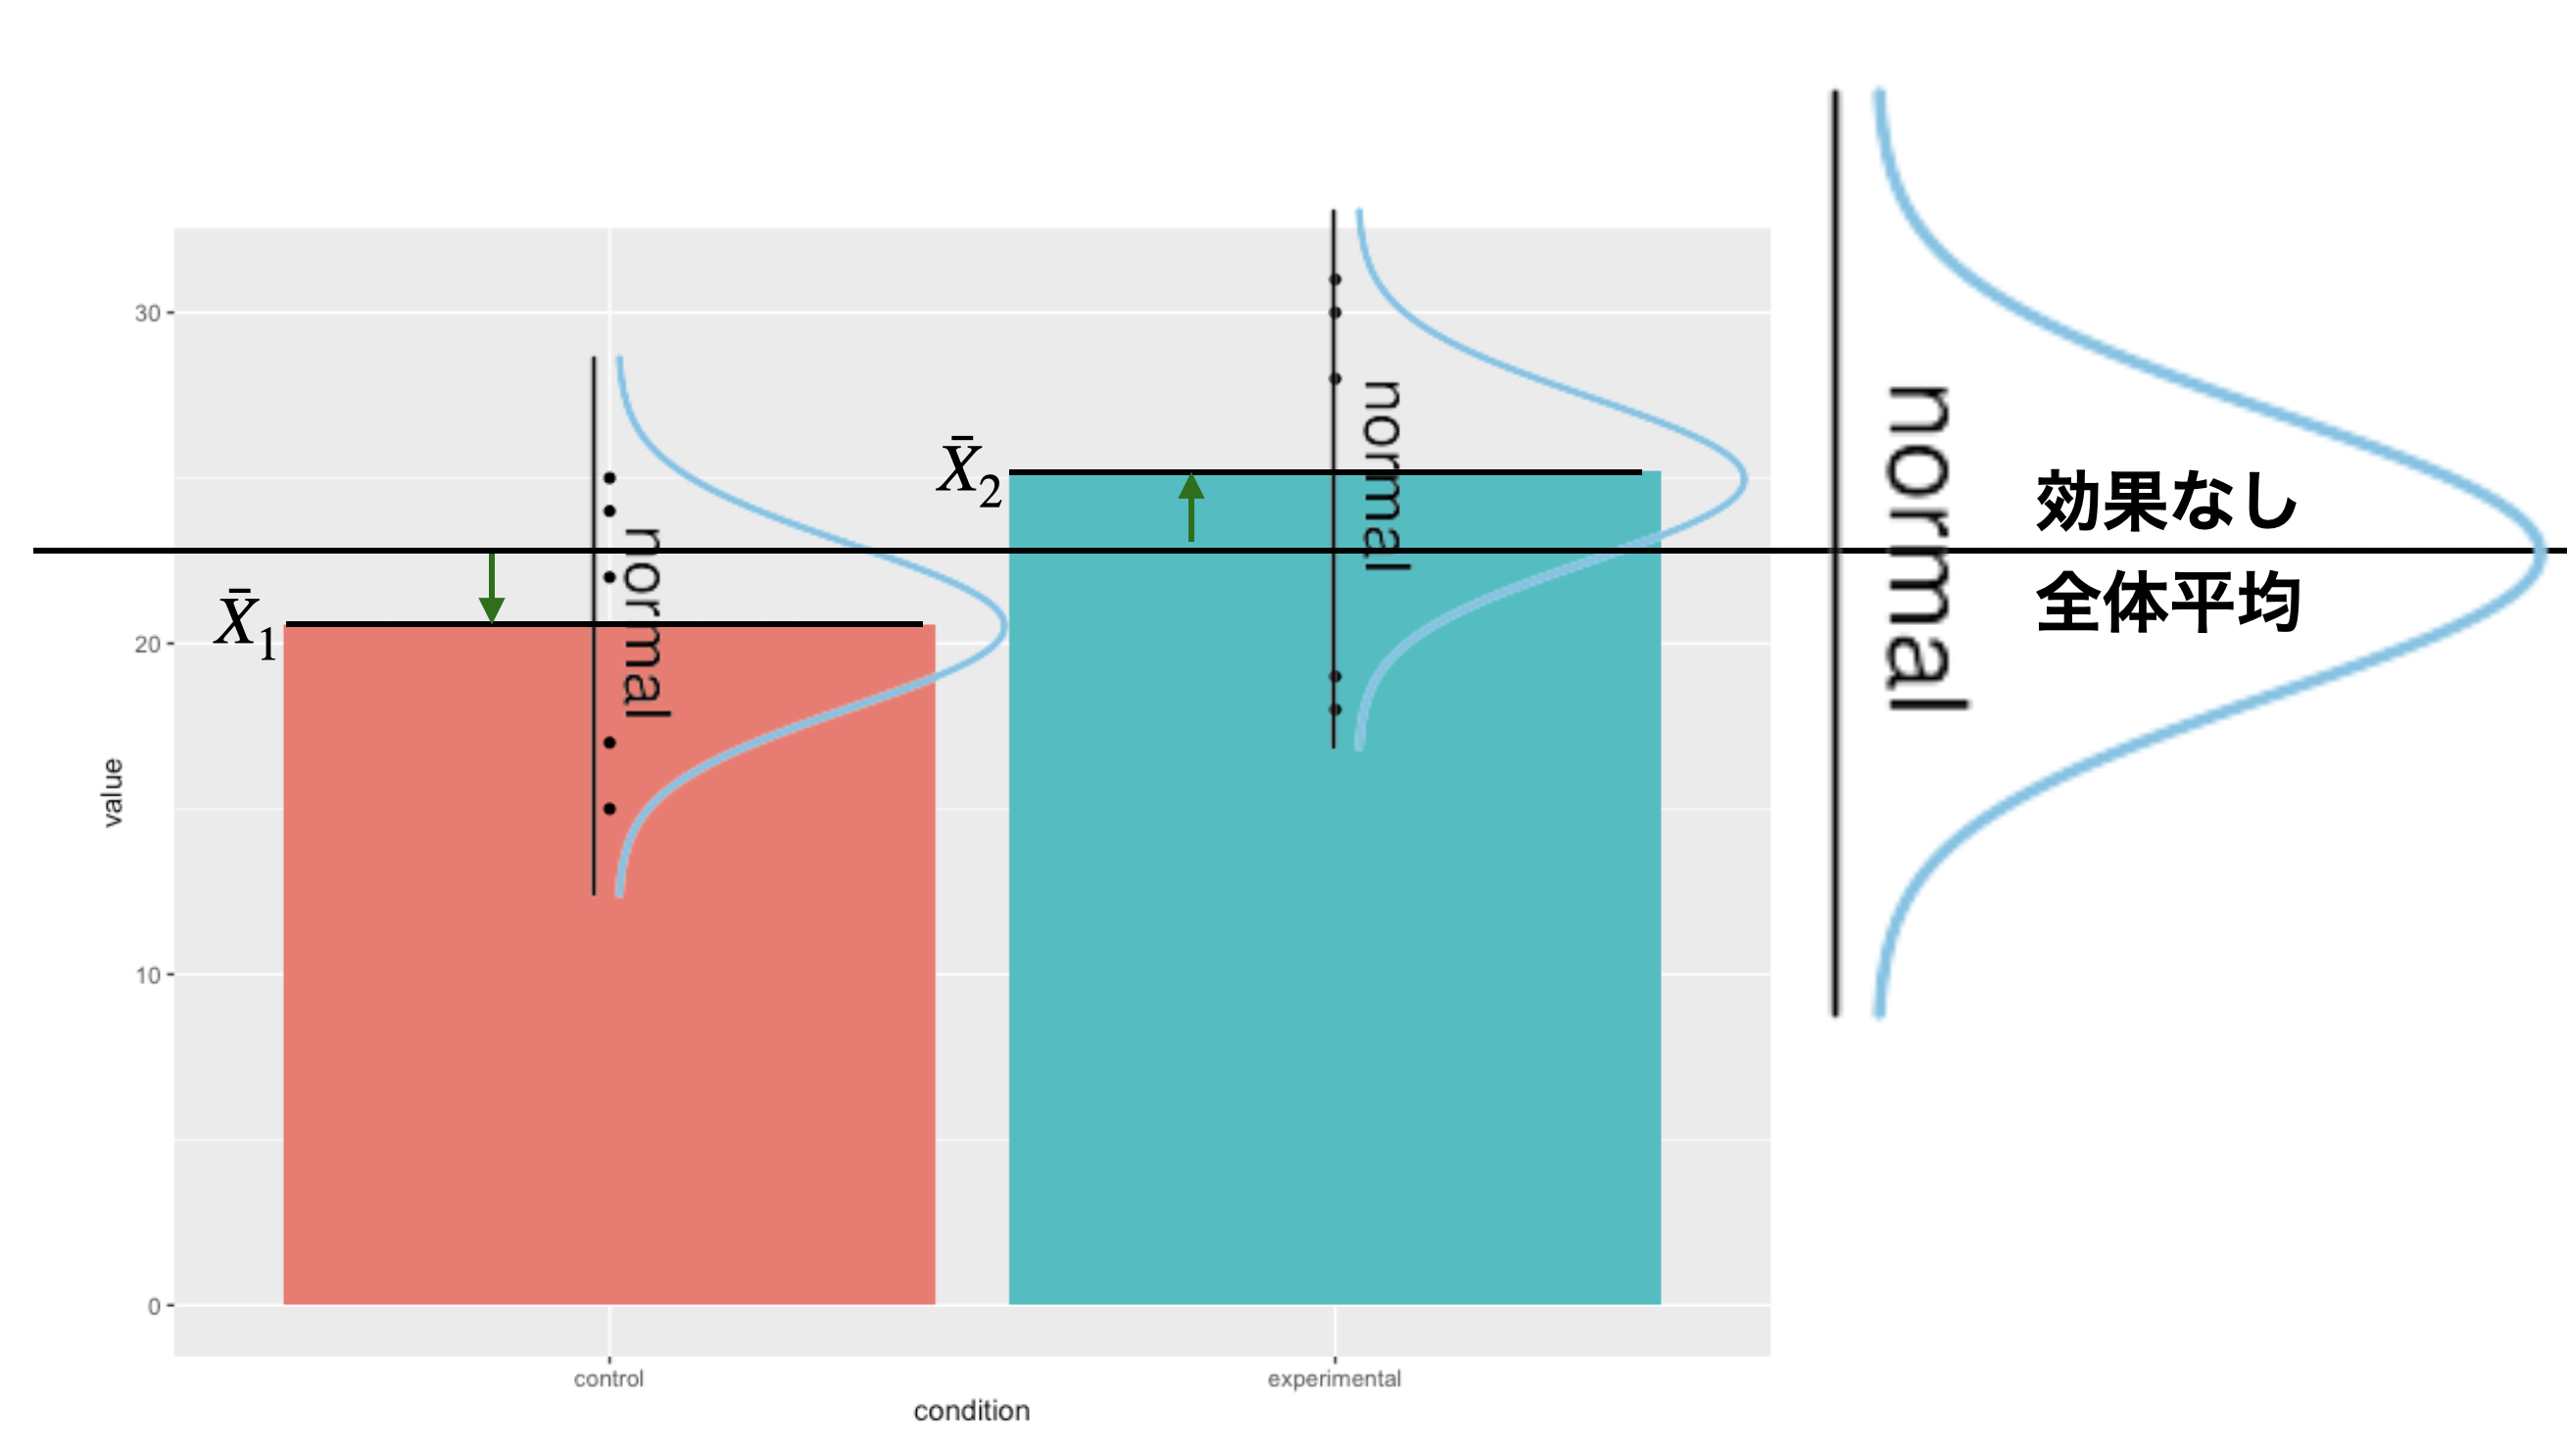
\includegraphics[keepaspectratio,width=0.8\linewidth]{figures/19_Ftest/two_levels_norm.png}
	\caption{効果がなければ全体平均に同じ。群の効果は相対的に平均値をずらす。}
	\label{fig:19_02}
\end{figure}

さて，群ごとの平均は次のように書くことができます。
\[ \bar{X}_1 =\frac{1}{5} \sum_{i=1}^5 X_{i1} \]
\[ \bar{X}_2 =\frac{1}{5} \sum_{i=1}^5 X_{i2} \]
また，全体平均次のように書くことができます\footnote{gmはgrand meanの略です。}。
\[ \bar{X}_{gm} = \frac{1}{10} \sum_{i} \sum_{j} X_{ij} \]
これは標本を使った平均値ですが，本来は推定したい(群間の差がない)母平均について議論したいところです。$\bar{X}_{gm}$は母平均の推定値として使い道はありますが，理想化・抽象化して語れるのがモデルの良いところですから，ここでは全体平均を未知数を表すギリシア文字$\beta$をつかって$\beta_0$としておきましょう。

さて次に，群わけの効果を$\beta_1$としましょう。すると各群の平均のモデルは
\[ \mu_1= \beta_0 + \beta_1 \]
\[ \mu_2 = \beta_0  -\beta_1 \]
と表すことができます。左辺も各群の母平均なので，未知数を表すギリシア文字になっています。

つづいて，ここでの個人差はこの実験で制御できない誤差であり，群平均を中心にどういう向きで出るかわからないものですから，このことを表現するなら，
\[ X_{ij} = \mu_j + \varepsilon_{ij} \]
ということになります。これらを組み合わせると，
\[ X_{i1} = \beta_0 + \beta_1 + \varepsilon_{i1} \]
\[ X_{i2} = \beta_0 - \beta_1 + \varepsilon_{i2} \]
と書くことができます。ここで一工夫。$\beta_1$にプラス，マイナスの符号がついているのは，$+1,-1$を掛け算していると考えてみましょう。この符号を決めているものを$X_{1}=+1,X_{2}=-1$と表したとすると，まとめて次のように書くことができます。
\begin{equation}
	\label{eq:19_01}
	X_{ij} = \beta_0 +  \beta_1 X_{j} + \varepsilon_{ij}
\end{equation}

これで線形モデルと同じ形になりました。$X_j$はダミー変数と呼ばれるもので，2つの群を区別するために使われています。$j=1$ならば$X_j=+1$，$j=2$ならば$X_j=-1$となります。

1つの共通の正規分布。2つの群に分かれない，同じ正規分布。そろそろ帰無仮説検定と繋がってきたのではないでしょうか。効果がない，というのはまさに，帰無仮説のことですよね。つまり帰無仮説は，$\beta_1=0$という傾きゼロの直線，図\ref{fig:19_02}では群平均を横切っている，横一線の線形モデルだったのです。平均値の差の検定というのは，群平均が横一直線＝傾きゼロではないよ，という結論を出すためのロジックであり，比較される対立仮説は「傾きゼロでない何か」というモデルです。
\begin{itemize}
	\item 帰無仮説H0: $\mu_1 = \mu_2$ $\to$ 線形モデルにおける傾きの係数$\beta_1=0$
	\item 対立仮説H1: $\mu_1 \neq \mu_2$ $\to$ 線形モデルにおける傾きの係数$\beta_1\neq 0$
\end{itemize}
帰無仮説が傾きゼロという一点ばりに対し，対立仮説はゼロ以外であれば何でも良いというラフなモデルです。ですから帰無仮説が棄却されたとしても「差がなくはない」という程度のもので，「じゃあゼロでない，何なのか」ということまでは強く主張できません。帰無仮説検定は補助的に使いつつ，実質はどのように傾いているのか，差の信頼区間はどの程度あるのか，効果量(標準化された平均値の差)は大きいのかといった，実質的な大きさを考えることが重要です。

\section{一要因Betweenデザインの検定}
この話が3水準以上になるとどうなるのでしょうか？
これも，基本的には線形モデルの延長で考えることができます。先ほどの表\ref{tbl:19_01}のようなデータがあったとしましょう。それぞれの群平均は，$\bar{X}_1 = 5.5,\bar{X}_2 = 6.0,\bar{X}_3 = 4.25$であり，全体平均は$\bar{X}_{gm}= 5.25$になります。
帰無仮説検定の文脈で考えれば，帰無仮説は「母平均に差がない」という仮説になりますから，記号で言えば$\mu_1 = \mu_2 = \mu_3$になります。
線形モデルで考えれば，図\ref{fig:19_03}にあるように，傾きのない線形モデル，つまり$X_{ij} = \bar{X}_{gm} + \varepsilon_{ij}$の横一線ということになります。

\begin{figure}[h]
	\centering
	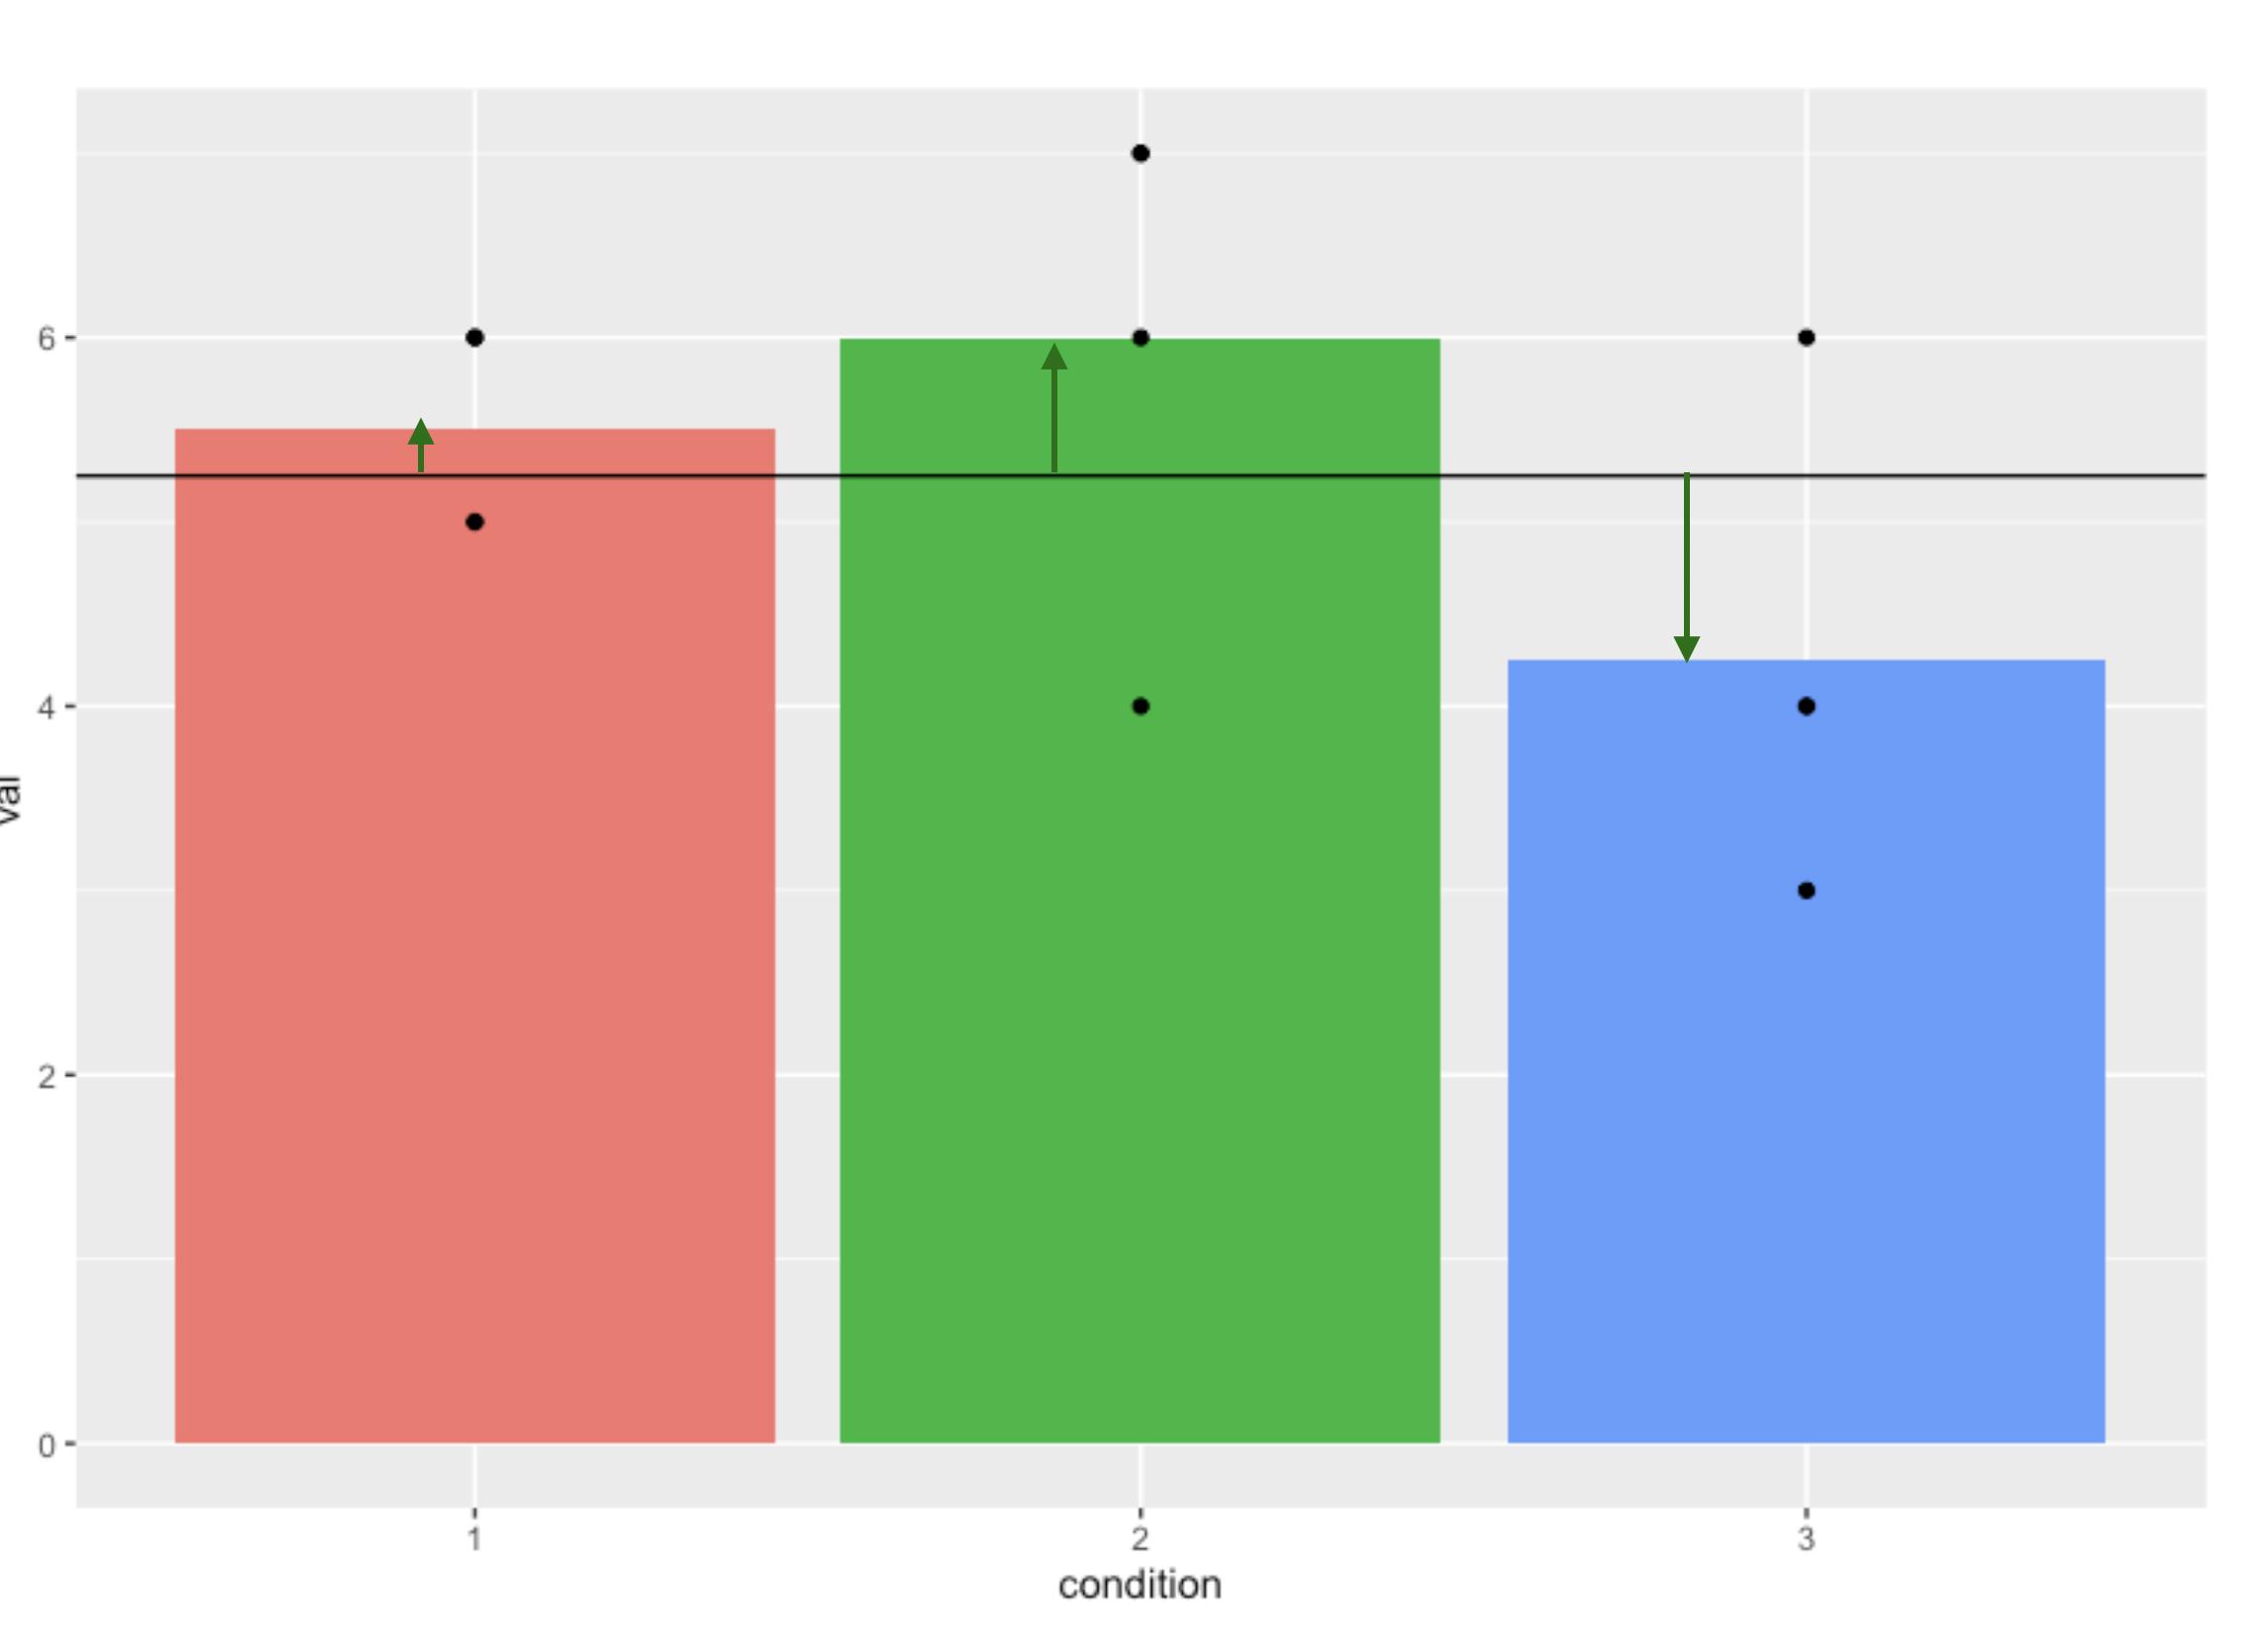
\includegraphics[keepaspectratio,width=0.8\linewidth]{figures/19_Ftest/three_levels.png}
	\caption{表\ref{tbl:19_01}を可視化したもの。全体平均からの矢印は群効果の大きさ}
	\label{fig:19_03}
\end{figure}

対立仮説は帰無仮説の否定ですから，横一線の直線ではない(傾きがある)，あるいは母平均のどこかに差がある，というものになります。横一線ではない，という話ではありますが，右上がりの直線なのか，左下りの直線なのか，という話は一概にできないことに注意してください。というのも，横軸の水準1,2,3は名義尺度水準に過ぎないからです。水準1,2,3が「統制群」「操作Aをした群」「操作Bをした群」であったとして，統制群が1である理由はとくになく，2でも3でも構いません。\underline{\keytermL{名義尺度水準}{めいぎしゃくどすいじゅん}は，対象と数字が一対一対応している}ことがその要件であって，数字の並びに意味がないからです。図\ref{fig:19_03}を見ると，水準1から2に向けては右上がり，水準2から3に向けては右下がりになって，一本の直線では表現できないですね。ただこれの並びを変えて，水準3,1,2の順番にすると右上がりの直線をあてがうことが可能です(図\ref{fig:19_04})。もちろん水準2,1,3の順にして右下がりの直線を当て嵌めても構いません。いずれもデータの持つ情報は同じです。ですから，対立仮説としては「横一線ではない」「母平均が同じではない」とするに留めましょう。

\begin{figure}[h]
	\centering
	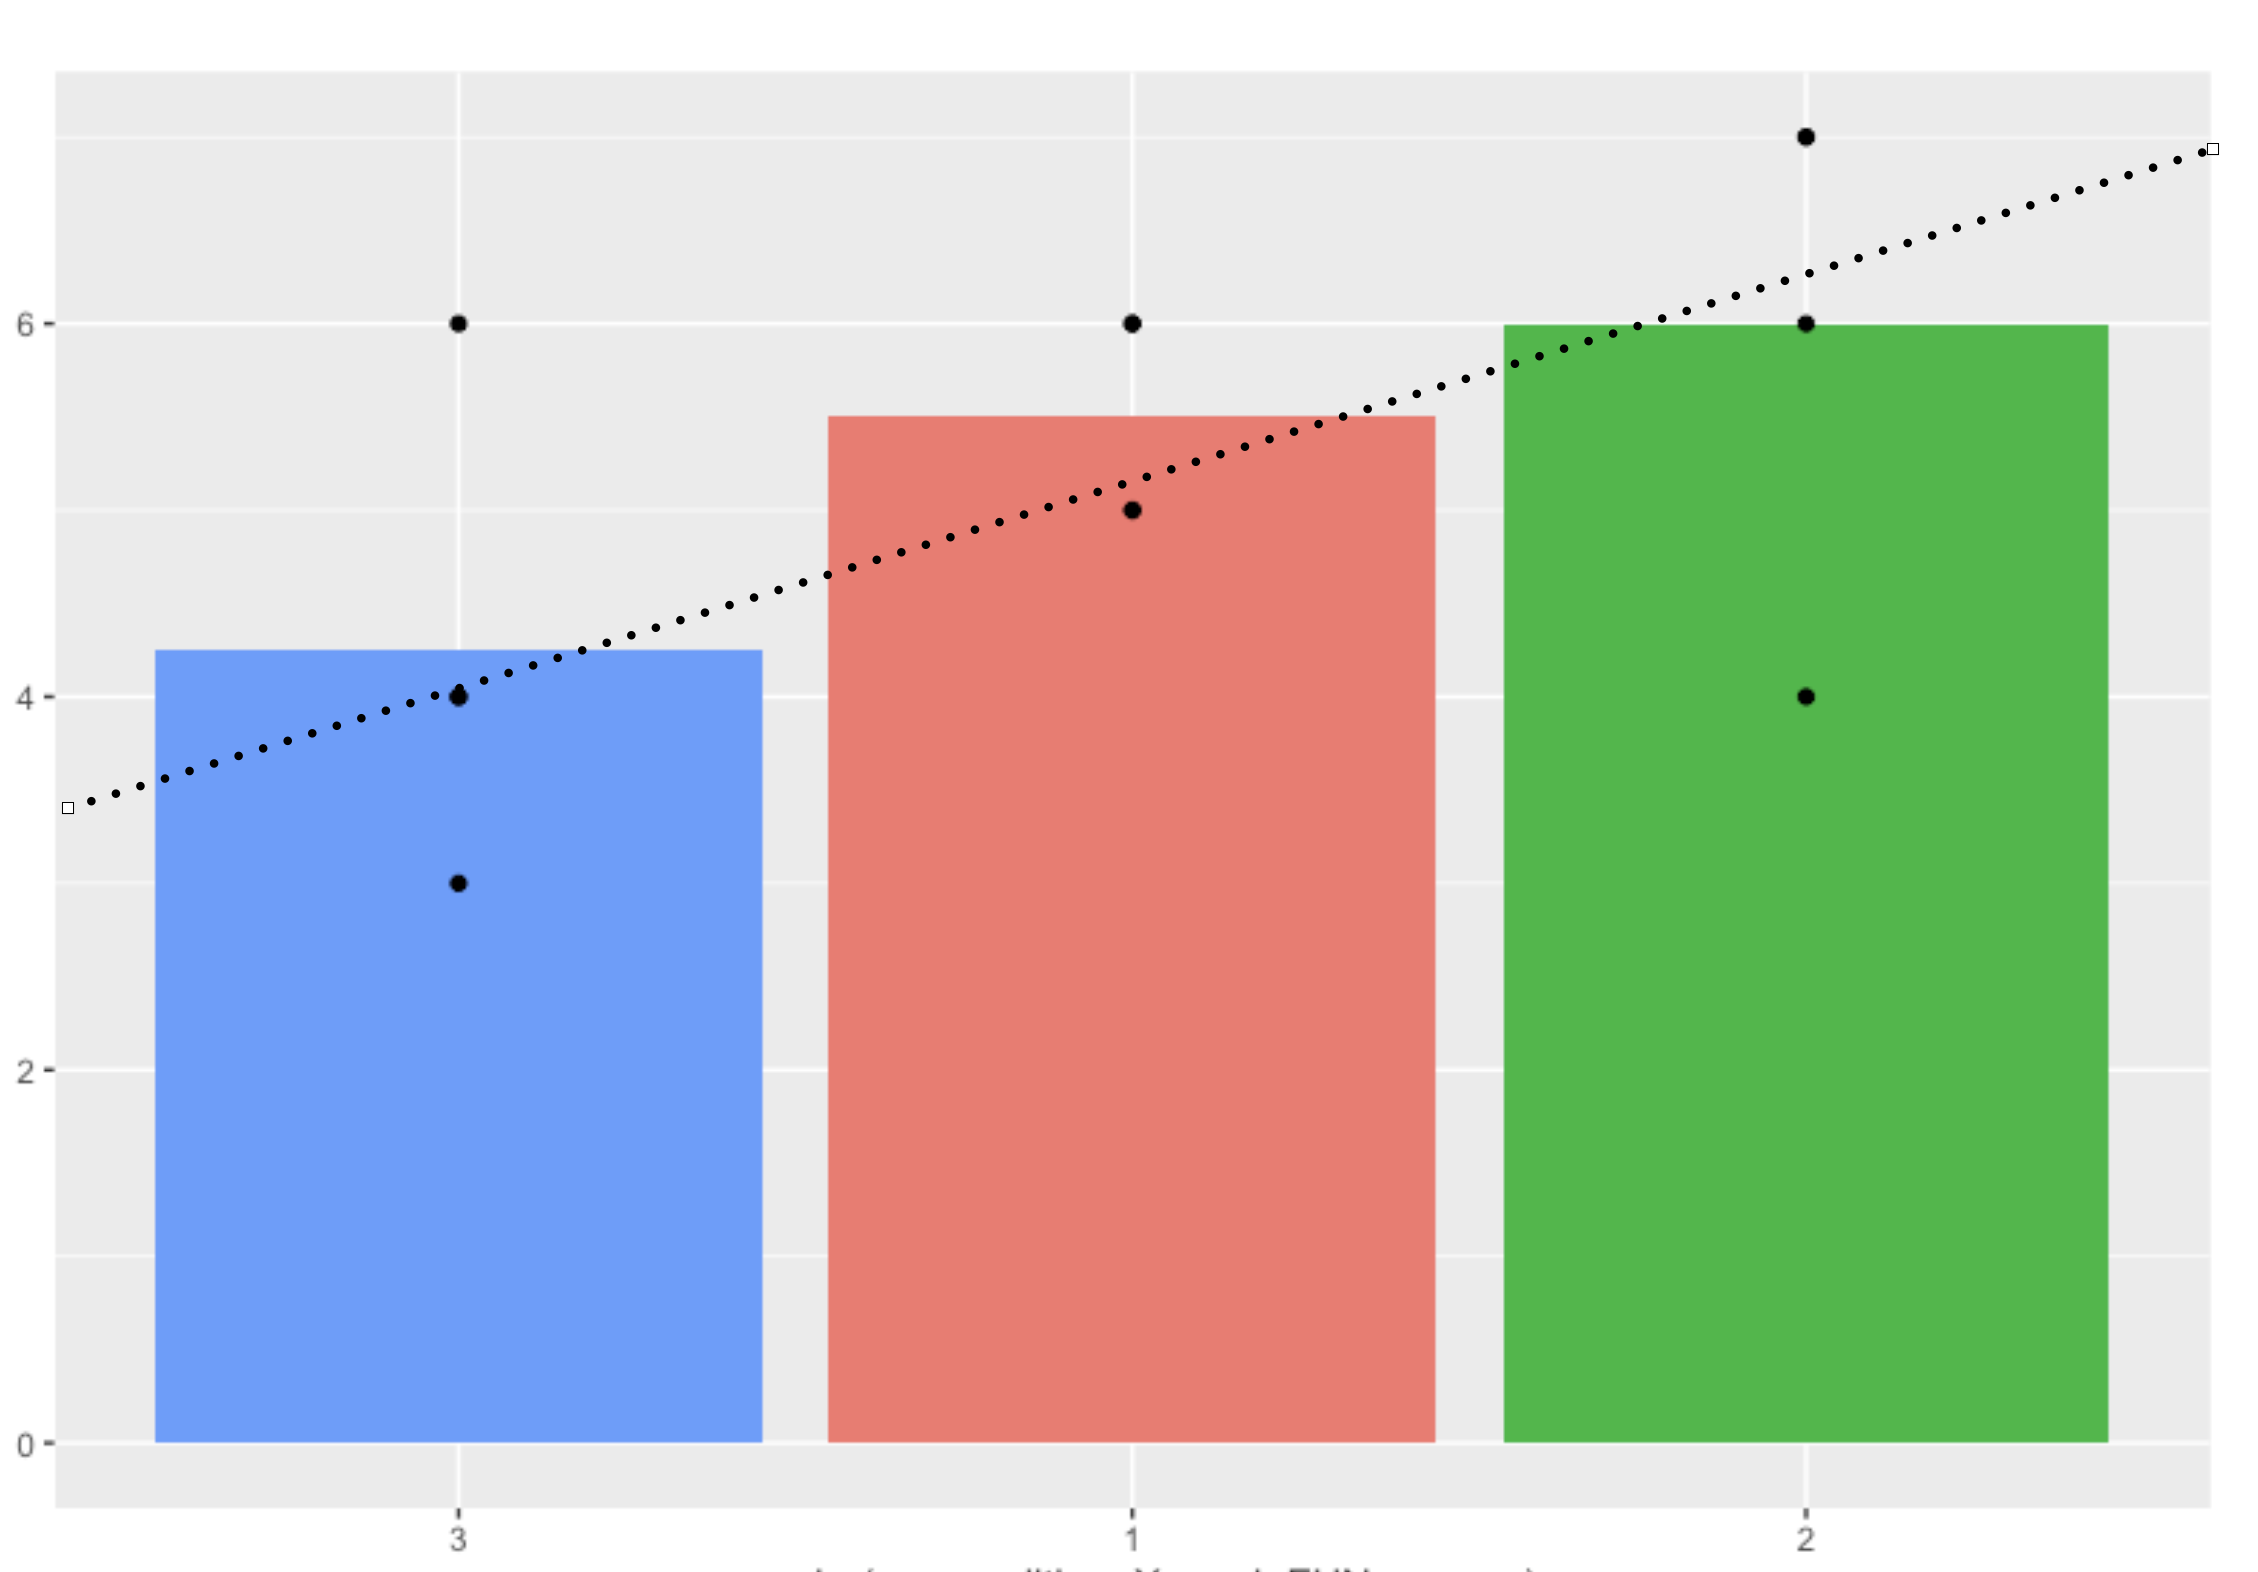
\includegraphics[keepaspectratio,width=0.8\linewidth]{figures/19_Ftest/three_levels2.png}
	\caption{横軸は並べ替えても構わない}
	\label{fig:19_04}
\end{figure}

\begin{itemize}
	\item 帰無仮説H0: $\mu_1 = \mu_2 = \mu_3 $ $\to$ 線形モデルにおける傾きの係数$\beta_1=0$
	\item 対立仮説H1: H0ではない。 $\to$ 線形モデルにおける傾きの係数$\beta_1\neq 0$
\end{itemize}

このように，水準が増えても同じ線形モデルとして表現できることがわかりました。要因の数が増えても同じです。説明変数が2つになりますので，散布図が3次元になり，直線が平面に変わるなどの違いはありますが，本質的に「母平均がすべて等しい＝平面が水平」という仮説に対する検定を行っていることになります。

\section{Rで分散分析をやってみよう}
さて，では理屈はここまでにして，実際に手を動かして計算してみましょう。といっても群ごとに平均を出したり，平方和を計算したり，そこから平均平方を作って比を計算して・・・というのはどう考えても大変。Rにやらせましょう。

流石にそろそろなれてきたとは思いますが，一応念のため，作業を始める前の最初のステップについて書いておきます。
\begin{enumerate}
	\item \textbf{RStudioの起動:}RStudioを起動してください。パッケージのインストールをするときなど，管理人権限が必要になるケースがあります。
	\item \textbf{プロジェクトを開く:}プロジェクトは前回作成した物で良いと思います。同じフォルダの中で，スクリプトファイルだけ変えれば良いでしょう。メニューからプロジェクトを開き(FIle$\to$Open Project)，RStudioの右上などで，プロジェクトが開いていることを確認しましょう。
	\item \textbf{Rスクリプトを開く:}今日のコードを書くためのRスクリプトファイルを準備します。\verb|File > NewFile > R Script|と進み，何も書いてないRスクリプトの画面を表示させてください。真っ白いファイルが開いたら問題ありません。
\end{enumerate}
準備ができたらスクリプトを書いていきましょう。と，その前に，Rで要因計画を扱うときのポイントである「変数の型」について説明しておきます。
\subsection{数の型}
繰り返しお話ししていますように，前期でやった回帰分析と今回扱う要因計画とは，線形モデルという同じ形をしています。違うところがあるとすれば，回帰分析の説明変数が連続的であるのに対し，要因計画の説明変数は離散的(カテゴリカル)であるということです。ですから，Rで分析する時も関数の形は同じであっても，変数の種類が違うということを明らかにしておかなければなりません。

Rにはいろいろな数字のタイプがあります。オブジェクトにいろいろな変数を格納できますが，その格納された変数のタイプには，次のような種類があります。
\begin{description}
	\item[numeric] 数字。加減乗除などの対象になるもの。尺度水準で言えば\keytermL{間隔尺度水準}{かんかくしゃくどすいじゅん}か\keytermL{比率尺度水準}{ひりつしゃくどすいじゅん}にあたるもの。
	\item[factor] ファクター型。訳して要因型ということもある。要因計画の「要因」です。この変数は数字とそれにつけるラベルとの組み合わせからなります。尺度水準で言えば\keytermL{名義尺度水準}{めいぎしゃくどすいじゅん}です。
	\item[orderd factor] 順序付きファクター型。ファクター型の特殊系で，中についている数字に順序情報がある物。尺度水準で言えば当然\keytermL{順序尺度水準}{じゅんじょしゃくどすいじゅん}に該当します。あまり使われることはないけど。
	\item[chr] 文字型(Character)。一見ファクター型と見分けがつかないこともあるが，こちらは内部に対応する数字があるわけでもなく，ただの文字。シングルクォーテーション，ダブルクォーテーションで括ったものが変数に渡されるとこの型になる。
	\item[logical] 論理型。\textit{TRUE}か\textit{FALSE}の2つの値しか持たない。\textit{TRUE}は$1$に，\textit{FALSE}は$0$に対応している。名義尺度水準の特殊な型で，オプションのスイッチオン・オフなどをこれで表したりする。大文字で書く\texttt{TRUE}や\texttt{FALSE}，あるいはそれらの一文字目\texttt{T}や\texttt{F}はこの型のラベルとして予約されているので\footnote{予約語といい，他にも何もないことを表す\texttt{NULL}や，無限大を表す\texttt{Inf}，欠測値を表す\texttt{NA}などがある。数学定数\texttt{pi}も予約語の1つ。}，オブジェクト名などにしない方が良い。
\end{description}
これらの型を確認するには，オブジェクトの仕組みがどうなっているかを調べる必要があります。調べるのは\texttt{str}関数で，これを使うとオブジェクトの中身がわかるようになっています。

次のコード，\texttt{code:\ref{code:19_01}}を入力してみてください。
\begin{lstlisting}[language=c++,label={code:19_01},caption={オブジェクトに代入}]
obj <- data.frame(
    list(name=c("kosugi","yamada","ueda"),
        gender = c(1,2,1),
        height = c(167,170,180),
        weight = c(60,70,80))
)
str(obj)
\end{lstlisting}
\paragraph{コード解説}
\begin{description}
	\item[1-6行目] データフレームを作って\texttt{obj}オブジェクトに代入している。
	\item[7行目] \texttt{obj}オブジェクトの構造を確認
\end{description}

さて，最後の7行目を実行すると，コンソールに次のように出力されていると思います(\texttt{Rの出力\ref{RS:out19_01}})。
\begin{Rscreen}{データフレームの中身}{out19_01}
	\begin{verbatim}
> str(obj)
'data.frame':	3 obs. of  4 variables:
 $ name  : chr  "kosugi" "yamada" "ueda"
 $ gender: num  1 2 1
 $ height: num  167 170 180
 $ weight: num  60 70 80
\end{verbatim}
\end{Rscreen}
ここにあるように，\texttt{obj}オブジェクトの\texttt{name}変数はchr型で，他の3つの変数は数値型(numeric)である，というのが示されています。ここで性別\texttt{gender}を因子型にしてみましょう(\texttt{code:\ref{code:19_02}})。

\begin{lstlisting}[language=c++,label={code:19_02},caption={因子型にする}]
obj$gender <- factor(obj$gender,label=c('male','female'))
\end{lstlisting}

これの出力は\texttt{Rの出力\ref{RS:out19_02}}のようになります。
\begin{Rscreen}{変数を因子型にした}{out19_02}
	\begin{verbatim}
> str(obj)
'data.frame':	3 obs. of  4 variables:
$ name  : chr  "kosugi" "yamada" "ueda"
$ gender: Factor w/ 2 levels "male","female": 1 2 1
$ height: num  167 170 180
$ weight: num  60 70 80
\end{verbatim}
\end{Rscreen}
ここに示されているように，性別がファクター型になり，それは2つの水準を持っている。それぞれに「male」「female」というラベルがついている，ということがわかります。

このfactor型にしておくというのは，Rが名義尺度水準の変数なんだなと理解したことになりますので，これで回帰分析をするとOKということになります。逆にfactor型にしておかないと，量的変数として普通の回帰分析をしてしまうので，正しくない結果になります\footnote{具体的には，3水準に1,2,3という量的な数字を割り振って分析するということは，$1<2<3$という順序性と2-1=3-2という等間隔性を持たせたことになります。要因計画の可視化の時に，横軸は入れ替え可能(順序性がない)だったことを思い出してください。}。

\section{一要因Between計画の実際}
ではまず一要因Between計画の話から。何度も例として使っている，表\ref{tbl:19_01}のデータを使います。\texttt{code:\ref{code:19_03}}のようにデータフレームを組み上げます。

\begin{lstlisting}[language=c++,label={code:19_03},caption={データの準備}]
# データフレームを組み上げる
Example1 <- data.frame(id = 1:12,
                       condition = rep(1:3,each=4),
                       value = c(6,6,5,5,7,4,7,6,4,3,4,6))
# 要因型にする
Example1$condition <- factor(Example1$condition,
                             labels = c("control","exp1","exp2"))
\end{lstlisting}

\paragraph{コード解説}
\begin{description}
	\item[1-3行目] データフレームを作っています。IDは被験者番号です。12人それぞれに異なる数字を振っています。条件conditionは3種類，各4人分(\texttt{rep(1:3,each=4)})，最後の従属変数(value)は手入力するしかありません。
	\item[5-7行目] 条件変数を要因型にしています。ラベルは統制群(control)と実験群1(exp1)，実験群2(exp2)としています。
\end{description}

\subsection{線形モデルとして分析}
線形モデルとしての分析は，前期でやったように\texttt{lm}関数を使います(\texttt{code:\ref{code:19_04}})。

\begin{lstlisting}[language=c++,label={code:19_04},caption={lm関数で分析}]
result.lm1 <- lm(value~condition,data=Example1)
summary(result.lm1)
\end{lstlisting}

1行目が\texttt{lm}関数を使っていて，結果を\texttt{result.lm1}オブジェクトに入れているところです。従属変数と独立変数をチルダ\verb|~|で繋げているところ，思い出してください。2行目はこの結果の出力になります。結果は\texttt{Rの出力\ref{RS:out19_03}}のように示されているはずです。
\begin{Rscreen}{lm関数の出力}{out19_03}
	\begin{verbatim}
Call:
lm(formula = value ~ condition, data = Example1)

Residuals:
   Min     1Q Median     3Q    Max 
-2.000 -0.500 -0.125  0.625  1.750 

Coefficients:
              Estimate Std. Error t value Pr(>|t|)    
(Intercept)     5.5000     0.5713   9.627 4.91e-06 ***
conditionexp1   0.5000     0.8079   0.619    0.551    
conditionexp2  -1.2500     0.8079  -1.547    0.156    
---
Signif. codes:  0 ‘***’ 0.001 ‘**’ 0.01 ‘*’ 0.05 ‘.’ 0.1 ‘ ’ 1

Residual standard error: 1.143 on 9 degrees of freedom
Multiple R-squared:  0.3562,	Adjusted R-squared:  0.2131 
F-statistic: 2.489 on 2 and 9 DF,  p-value: 0.1379
\end{verbatim}
\end{Rscreen}
これを見ると，切片\texttt{(Intercept)}の推定値が5.5，次に2つの説明変数の係数が書いてあります。文字が連なっているのでわかりにくいかもしれませんが，それぞれ\texttt{condition}と\texttt{exp1}の関係，\texttt{condition}と\texttt{exp2}の関係を表しています。図\ref{fig:19_05}を見ると結果の意味は分かり易いと思います。
\begin{figure}[ht]
	\centering
	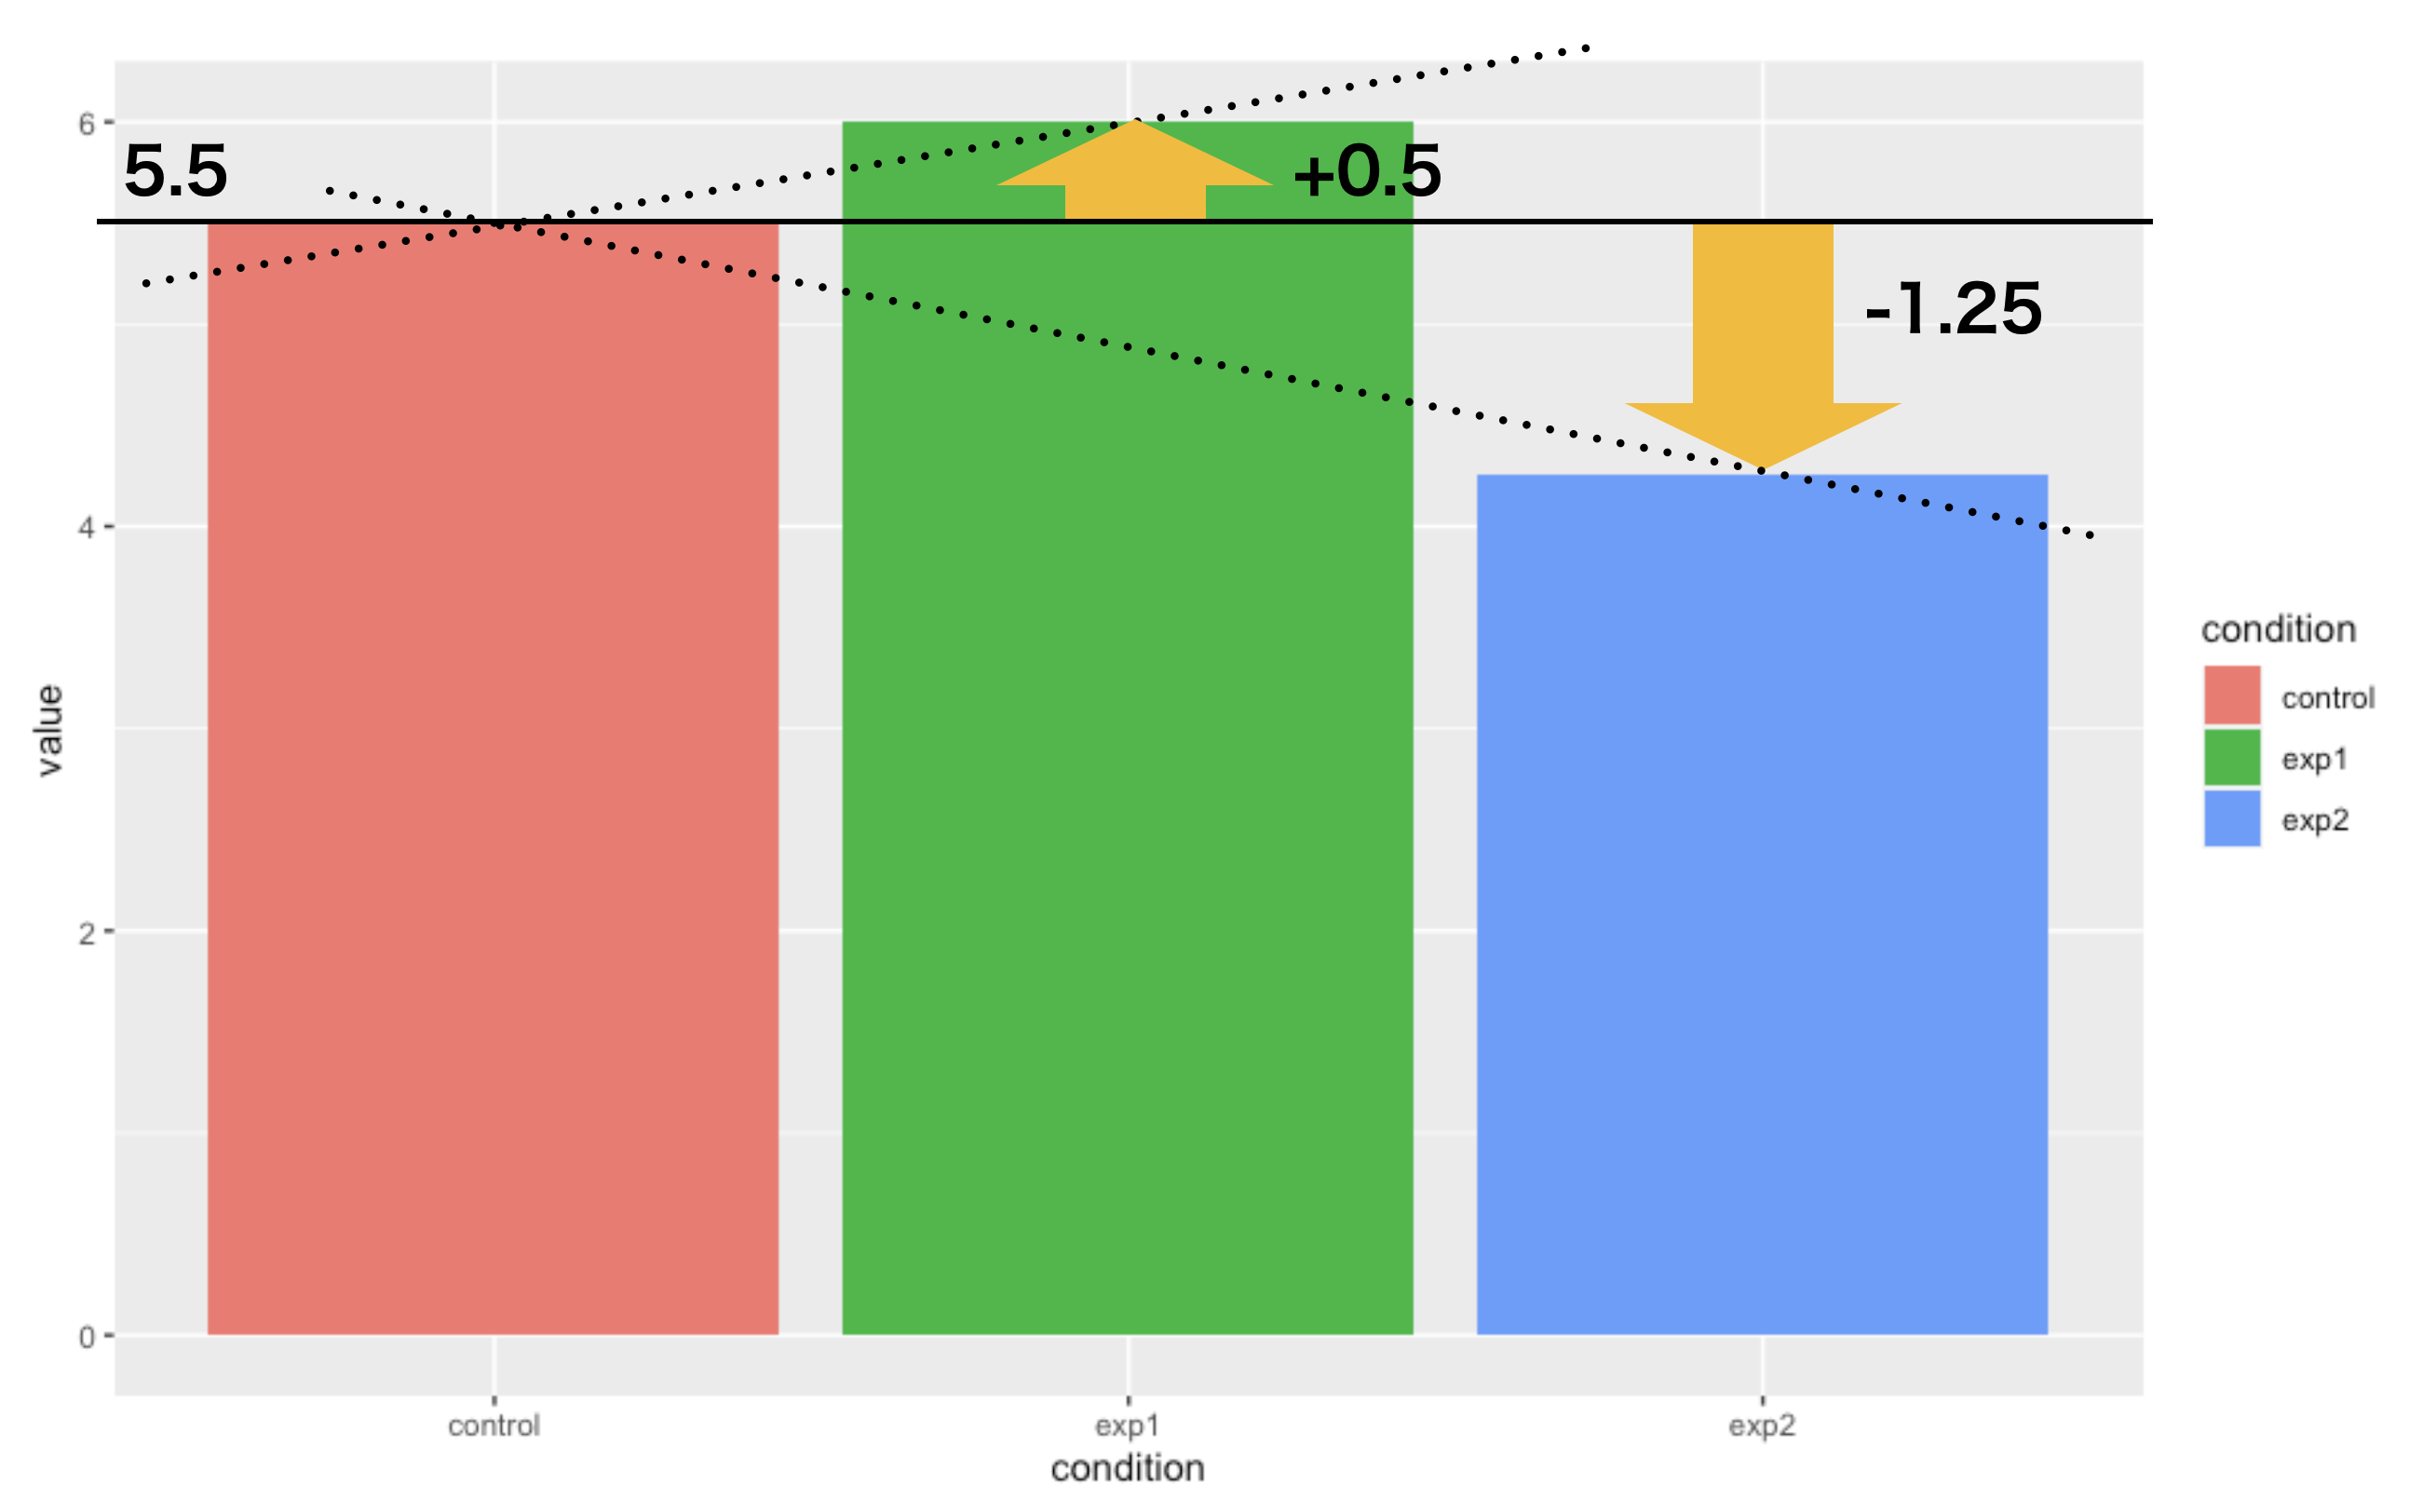
\includegraphics[keepaspectratio,width=0.8\linewidth]{figures/19_Ftest/linear_model.png}
	\caption{線形モデルとして分析した結果の意味するもの}
	\label{fig:19_05}
\end{figure}

線形モデルの式は，次のようになります。
\[ X_{ij} = \beta_0 + \beta_j + \varepsilon_{ij} \]
ここで$\beta_0$は全体平均でした。全体平均を基本として，各水準に対する効果$\beta_j$がどうなったか，というモデル化でしたが，ここでは
\[ X_{ij} = \bar{X}_1 + \beta_j + \varepsilon_{ij} \]
という形になっています(図\ref{fig:19_05})。本質的に違うものではありません。統制群に比べて実験群1の平均値は$+0.5$，実験群2は$-1.25$の平均値の違いがあるのだな，と思っていただければ結構です。その後ろにStd.Errorや$t$値が出ていますが，これらは推定された回帰係数の標準誤差および，係数が$0$であるという帰無仮説を棄却できるかどうかの検定結果が出ています\footnote{各群の母平均の推定値でもありますが，各群について一変数の$t$検定をしているのではなく，これら線形モデル全体として(他の説明変数に条件づけられた分布の中で)標準誤差を計算します。詳しくは\textcite{Haebara200206}のp.118を参照してください。}。

線形モデルですから，モデルの適合度(\texttt{Multiple R-squared, Adjusted R-squared})なども出ていますが，それよりも最後の一行，この線形モデル全体の検定結果が出ています。これは要因計画のもう1つの切り口，分散分析による結果と同じものです。では分散分析の視点からこの分析結果を見てみましょう。

\subsection{帰無仮説検定として分析}
要因計画の帰無仮説検定版，つまり分散分析の結果ですが，線形モデルと同じなので今回得られた出力をすこし変えるだけで対応できます。最も単純には，先ほどの線形モデルの結果を\texttt{anova}関数に入れると，分散分析表が次のように示されます(\texttt{code:\ref{code:19_05}},\texttt{Rの出力\ref{RS:out19_04}})。


\begin{lstlisting}[language=c++,label={code:19_05},caption={分散分析としてみる}]
anova(result.lm1)
\end{lstlisting}


\begin{Rscreen}{分散分表の出力}{out19_04}
	\begin{verbatim}
Analysis of Variance Table

Response: value
          Df Sum Sq Mean Sq F value Pr(>F)
condition  2   6.50  3.2500  2.4894 0.1379
Residuals  9  11.75  1.3056   
\end{verbatim}
\end{Rscreen}

ここから，$F(2,9)=2.4894,p=0.1379$で統計的に有意な差はみられなかった，と判断できます。これらの数字，どこをどう読み取ったのか確認してください。

ちなみに，同じことですが分散分析関数\verb|aov|というのもあります。こちらを使うと，直接分散分析表が出力されます(\texttt{code:\ref{code:19_06}})。

\begin{lstlisting}[language=c++,label={code:19_06},caption={aov関数で実行する}]
result.aov <- aov(value~condition, data = Example1)
summary(result.aov)
\end{lstlisting}

\begin{Rscreen}{分散分表の出力その2}{out19_05}
\begin{verbatim}
            Df Sum Sq Mean Sq F value Pr(>F)
condition    2   6.50   3.250   2.489  0.138
Residuals    9  11.75   1.306 
\end{verbatim}
\end{Rscreen}
どちらの方法を使ってもらっても構いません。

さて，今回は統計的に有意であるとは言えませんでしたが，もし統計的に有意であるという結果であれば，どの群とどの群が違うのか，ということを調べる必要があります。これを\keyterm{下位検定}{かいけんてい}{post-hoc analysis}や\keyterm{事後比較}{じごひかく}{post-hoc comparison}といいます。手法はいろいろな種類がありますが，Rでは\texttt{TukeyHSD}関数を使うのが簡単です(\texttt{code:\ref{code:19_07}})。

\begin{lstlisting}[language=c++,label={code:19_07},caption={事後比較}]
TukeyHSD(result.aov)
\end{lstlisting}

\begin{Rscreen}{事後比較の出力}{out19_06}
\begin{verbatim}
> TukeyHSD(result.aov)
  Tukey multiple comparisons of means
    95% family-wise confidence level

Fit: aov(formula = value ~ condition, data = Example1)

$condition
              diff       lwr       upr     p adj
exp1-control  0.50 -1.755792 2.7557916 0.8137078
exp2-control -1.25 -3.505792 1.0057916 0.3158385
exp2-exp1    -1.75 -4.005792 0.5057916 0.1311336
\end{verbatim}
\end{Rscreen}

もちろん最初に統計的に有意ではなかったのですから，ここでも群間の比較で統計的に有意な差は出ていません。
しかし，もし有意であった場合，この表の\texttt{p adj}列を見て，0.05より小さいものがあれば，その2つの群の平均値は統計的に有意に異なる，と判断できます。

また，効果量も計算しておきましょう。効果量は\texttt{effectsize}パッケージを使うと簡単に計算できます(\texttt{code:\ref{code:19_08}})。

\begin{lstlisting}[language=c++,label={code:19_08},caption={効果量の算出}]
library(effectsize)
epsilon_squared(result.aov)
\end{lstlisting}

効果量については他にも様々な指標(Cohen's f,$\eta^2,\omega^2$など\footnote{簡単に説明すると，Cohen's fは2群の効果量の多群版です。$\eta^2,\omega^2$は全体の分散のうち何\%が効果で説明されるかの指標。$\eta^2$は標本における寄与率であり，母集団の効果を過大評価してしまう可能性があるといわれています。$\omega^2$は$\eta^2$のその偏りを補正したものです。})がありますが，ここでは$\epsilon^2$を使っています。出力は\texttt{Rの出力\ref{RS:out19_06b}}のようになります。
\begin{Rscreen}{効果量の出力}{out19_06b}
\begin{verbatim}
For one-way between subjects designs, partial epsilon squared is
  equivalent to epsilon squared. Returning epsilon squared.
# Effect Size for ANOVA

Parameter | Epsilon2 |       95% CI
-----------------------------------
condition |     0.21 | [0.00, 1.00]	
\end{verbatim}
\end{Rscreen}

このようにして，複雑な計算もRのコードを使うと比較的簡単に実行できるのでした。

\section{課題}

\subsection{問題1：平方和の計算と分散分析}

ある研究者が，3つの異なる学習方法（方法A，方法B，方法C）がテスト成績に与える影響を調べるため，各方法に4名ずつ，計12名の学生を無作為に割り当てました。1週間後のテスト結果（100点満点）は表\ref{tbl:19_04}のようになりました。

\begin{table}[ht]
	\centering
	\caption{学習方法別のテスト成績}
	\begin{tabular}{cccc}
		\hline
		学生ID & 学習方法 & 成績 \\
		\hline
		1 & A & 75 \\
		2 & A & 80 \\
		3 & A & 70 \\
		4 & A & 85 \\
		5 & B & 82 \\
		6 & B & 88 \\
		7 & B & 85 \\
		8 & B & 89 \\
		9 & C & 68 \\
		10 & C & 72 \\
		11 & C & 70 \\
		12 & C & 74 \\
		\hline
	\end{tabular}
	\label{tbl:19_04}
\end{table}
このデータを用いて，次のRコードを書いて分散分析を実行したものを提出してください。
\begin{enumerate}
	\item データフレームを作成し，学習方法を因子型に変換するコードを書きましょう。
	\item \texttt{aov}関数を使って分散分析を実行し，結果を表示するコードを書きましょう。
	\item 結果を読み，統計的に有意であると判断して良いかどうか回答してください。回答はスクリプトの中に，コメントアウトして書いてください。
	\item 有意差があると判断した場合，TukeyのHSD検定を実行し，どの群間に有意差があるかを調べましょう。
	\item 効果量（$\epsilon^2$または$\eta^2$）を計算するコードを書きましょう。
\end{enumerate}

% # 1. データフレームを作成し，学習方法を因子型に変換する
% # ========================================

% # データの入力
% data_kadai <- data.frame(
%   student_id = 1:12,
%   method = rep(c("A", "B", "C"), each = 4),
%   score = c(75, 80, 70, 85,  # 方法A
%             82, 88, 85, 89,  # 方法B
%             68, 72, 70, 74)  # 方法C
% )

% # 学習方法を因子型に変換
% data_kadai$method <- factor(data_kadai$method,
%                             levels = c("A", "B", "C"),
%                             labels = c("方法A", "方法B", "方法C"))


% # 分散分析の実行
% result_aov <- aov(score ~ method, data = data_kadai)
% summary(result_aov)

% # 判断（コメント）
% # ========================================
% # F値 = 21.088, p値 = 0.00037 < 0.05
% #
% # 結論：
% # 有意水準5%で検定した結果，p値が0.05より小さいため，
% # 帰無仮説「3つの学習方法の母平均は等しい」を棄却する。
% # したがって，学習方法間に統計的に有意な差があると判断できる。
% # ========================================


% # 4. TukeyのHSD検定を実行
% # ========================================

% tukey_result <- TukeyHSD(result_aov)
% print(tukey_result)


% # 5. 効果量（η²）を計算する
% # ========================================
% library(effectsize)
%   print(eta_squared(result_aov))
%   print(omega_squared(result_aov))
%   print(cohens_f(result_aov))





\end{document}
